\expandafter\def\csname ver@breakurl.sty\endcsname{2013/04/10}\expandafter\def\csname opt@breakurl.sty\endcsname{hyphenbreaks}% skip breakurl (dvips only); Tectonic runs XeTeX
\documentclass[sn-basic,Numbered]{sn-jnl}
% Shared preamble for the Springer Nature (sn-jnl) versions: papers A and B. Load right after \documentclass{sn-jnl}.
\usepackage{amsmath,amssymb}
\usepackage{graphicx}
\usepackage{booktabs}
\usepackage{tabularx}
\usepackage{array}
\usepackage{xcolor}
\usepackage{tikz}
\usetikzlibrary{arrows.meta,positioning,fit,backgrounds,calc,shapes.geometric,shapes.misc}
\graphicspath{{../figures/}}
% sn-jnl loads breakurl, which expects pdfTeX/dvips; Tectonic runs XeTeX
\makeatletter\def\headerps@out#1{}\makeatother
\AtBeginDocument{\def\doi#1{\url{https://doi.org/#1}}}\providecommand\burl{\url}
% a result the overnight runs have not produced yet (papers/analysis/new_results.py fills it in)
\newcommand{\pending}{\textcolor{red}{[pending]}}
% a step that needs people (raters, reviewers, ethics); see papers/HUMAN_STUDIES.md
\newcommand{\humanpending}[1]{\textcolor{red}{[#1]}}
\tikzset{
  >={Stealth[length=1.8mm]},
  box/.style={draw, rounded corners=2pt, align=center, font=\scriptsize, minimum height=7mm, inner sep=2pt, fill=#1},
  box/.default=cyan!8,
  decision/.style={draw, diamond, aspect=2.2, align=center, font=\scriptsize, inner sep=1pt, fill=yellow!12},
  state/.style={draw, circle, align=center, font=\scriptsize, minimum size=12mm, fill=#1},
  state/.default=cyan!8,
  lab/.style={font=\tiny, align=center},
}
\newcolumntype{Y}{>{\raggedright\arraybackslash}X}

\newcommand{\numCasFalse}{3.7\%}
\newcommand{\numCasRisk}{93.5\%}
\newcommand{\numCasShare}{63\%}
\newcommand{\numCompCIPzero}{[0.969, 0.987]}
\newcommand{\numCompCIVzero}{[0.954, 0.979]}
\newcommand{\numCompCIVtwo}{[0.956, 0.982]}
\newcommand{\numCompPzero}{0.978}
\newcommand{\numCompVzero}{0.967}
\newcommand{\numCompVtwo}{0.970}
\newcommand{\numDiffPzero}{$-0.008$ [$-0.022$, $+0.004$]}
\newcommand{\numFilterDropped}{240}
\newcommand{\numFilterTotal}{533}
\newcommand{\numJailPzero}{6}
\newcommand{\numJailVzero}{1}
\newcommand{\numJailVtwo}{0}
\newcommand{\numLLMfalse}{4.8\%}
\newcommand{\numLLMmsMed}{416}
\newcommand{\numLLMmsNinety}{736}
\newcommand{\numLLMrisk}{94.8\%}
\newcommand{\numLeaksPzero}{4}
\newcommand{\numLeaksVzero}{0}
\newcommand{\numLeaksVtwo}{1}
\newcommand{\numPortPzero}{0}
\newcommand{\numPortVzero}{0}
\newcommand{\numPortVtwo}{0}
\newcommand{\numRPmissNoRecPzero}{66.7\%}
\newcommand{\numRPmissNoRecVzero}{55.3\%}
\newcommand{\numRPmissNoRecVtwo}{69.8\%}
\newcommand{\numRPmissRecPzero}{51.8\%}
\newcommand{\numRPmissRecVzero}{21.0\%}
\newcommand{\numRPmissRecVtwo}{24.4\%}
\newcommand{\numRPmissPzero}{55.8\%}
\newcommand{\numRPmissVzero}{43.3\%}
\newcommand{\numRPmissVtwo}{36.8\%}
\newcommand{\numRPnPzero}{231}
\newcommand{\numRPnVzero}{231}
\newcommand{\numRPnVtwo}{231}
\newcommand{\numSIfailPzero}{1}
\newcommand{\numSIfailVzero}{0}
\newcommand{\numSIfailVtwo}{0}
\newcommand{\numTurnsPzero}{294}
\newcommand{\numTurnsVzero}{294}
\newcommand{\numTurnsVtwo}{294}
\newcommand{\numWGemmaDep}{47.5\%}
\newcommand{\numWGemmaLLM}{91.5\%}
\newcommand{\numWQwenDep}{58.9\%}
\newcommand{\numWQwenLLM}{87.7\%}


\begin{document}

\title[Decide in Code, Voice with the Model]{Decide in Code, Voice with the Model: A Code-Governed Patient Model for an On-Device
Psychiatric Standardised Patient, Compared with a Prompt-Only Baseline}

% Author checks still to do: papers/HUMAN_STUDIES.md
\author*[1]{\fnm{Faaz Khan} \sur{Mohammad}}\email{faazkhn1000@gmail.com}
\author[1]{\fnm{Sanket} \sur{Salvi}}
\affil[1]{\orgdiv{Department of Computer Engineering and Technology}, \orgname{Dr.~Vishwanath~Karad MIT World Peace University}, \orgaddress{\city{Pune}, \state{Maharashtra}, \country{India}}}

\abstract{Language-model patients for psychiatric interview practice can invent symptoms and are unpredictable about suicidal thoughts, and
their reasons for sharing or withholding are hidden. We describe a patient model for Rapport, an on-device spoken standardised patient, in which
code makes every decision a clinician would audit: how the doctor's sentence changes trust and guardedness, which memories are open, and which
behaviours are allowed. One call to a local 4-billion-parameter language model (Gemma 4 E4B) puts the decision into words, and every sentence is
checked before it is spoken. We compared it with a prompt-only baseline: the same model given the whole case file and told to hide risk memories
until trust is built. On 14 held-out scripted conversations, each run with three seeds and judged by a model from another family, the primary
outcome, per-conversation accuracy against the case, was \numCompVtwo{} for the code-governed model and \numCompPzero{} for the baseline
(paired difference \textminus0.008, 95\% confidence interval \textminus0.022 to 0.004). Safety differed: the code-governed model failed no jailbreak or portrayal check
and always disclosed the death wish when it was due, while the baseline failed \numJailPzero{} jailbreak checks and once withheld the death wish.
Passing these checks is not a guarantee. When 77 reworded risk questions from a blind benchmark were asked in conversation at sufficient trust,
the code-governed model failed to disclose in \numRPmissVtwo{} of cases (baseline \numRPmissPzero), through missed matches and through answering
plan or means questions with the death wish. The clinical content has not been reviewed by a psychiatrist.}

\keywords{simulated patients, psychiatry education, large language models, patient safety, on-device AI, evaluation}

\maketitle

\section{Introduction}\label{sec:intro}
The psychiatric interview is learned by doing. A trainee has to notice slow speech and a lowered gaze, ask open questions, earn enough trust
for a patient to admit that some nights they wish they would not wake up, and then assess risk, all inside a timed examination station (an
OSCE \cite{harden1975osce}). Actors trained as standardised patients make this practice possible, but they are costly, not always available,
and hard to keep consistent between students \cite{piot2021simulation}.

Large language models (LLMs) can play a patient, and many research systems now do
\cite{chen2023llmempowered,wang2024patient,lee2025psyche,sabour2026patientact,sabour2026patienthub,louie2024roleplaydoh}; a 2026
meta-analysis found that AI virtual patients help psychiatric interview training \cite{kilincel2026meta}. Three problems matter most for a
medical system that students use unsupervised. The model makes things up: it invents symptoms or history to please the interviewer
\cite{chen2023llmempowered}, and simulated patients agree too easily unless resistance is designed in \cite{steenstra2025scaffolding,lee2025psyche}.
It is unpredictable where it matters most, such as whether a patient admits suicidal thoughts, and nobody can see why it shared or held
something back. And most systems run in the cloud, so a student's voice leaves the premises.

The common answer is a better prompt: give the model the case file and tell it how to behave. Our central claim is that this is not enough,
and that the decisions a clinician would audit should be taken out of the model altogether. We call this \emph{decide in code, voice with the
model}. The patient's state, which memories are open, how guarded it is and which behaviours it may use are computed by code we can read,
test and change; one model call per turn only writes the words, and every sentence is checked before it is spoken. We call the patient model
the \emph{Digital Twin}: an inspectable counterpart of one authored case file, mirrored live to the examiner. It is not a twin of a real
person, nor a model of the brain.

\textbf{Contributions.}
\begin{enumerate}
\item A code-governed patient model with explicit state, trust-locked memory, rule-based resistance, a decision layer that constrains the
model's output, and sentence checks before speech (Section~\ref{sec:model}).
\item A direct test of the central claim: the same model and case files with no code decisions (a prompt-only baseline), scored by the same
judges on the same held-out conversations (Sections~\ref{sec:method} and~\ref{sec:res-baseline}).
\item A measure of what safety gates miss: reworded risk questions from a blind benchmark asked inside real conversations, linking
conversation-level safety to the accuracy of memory matching (Section~\ref{sec:res-risk}).
\item Feature ablations and the defects found by an automated adversarial code review (Sections~\ref{sec:res-ablation}--\ref{sec:res-review}).
\end{enumerate}
A companion manuscript by the same authors studies the memory-matching step on its own.

\section{Related Work}\label{sec:related}
\textbf{Psychiatric AI patients.} Chen et al.\ built chatbots validated by clinicians for depression interviews \cite{chen2023llmempowered};
PATIENT-$\Psi$ bases patients on expert cognitive models with six conversation styles \cite{wang2024patient}; PSYCHE builds a Mental Status
Exam framework to evaluate assessment agents \cite{lee2025psyche}; PatientAct adds trust-gated memory, reactions and resistance
\cite{sabour2026patientact}; PatientHub collects many simulators \cite{sabour2026patienthub}; Roleplay-doh lets experts steer a patient with
written principles \cite{louie2024roleplaydoh}. EvoPatient improves patients through simulated practice and a checked library of past replies
\cite{du2024llms}. Patients with a body or voice include Voigt et al.\ \cite{voigt2025llmpowered} and SOPHIE \cite{haut2025ai}, and a randomised
trial found that simulation with structured feedback improved students' clinical decisions \cite{brugge2024llm}. Most of these systems control the
patient through the prompt, sometimes with several model calls per turn; PatientAct moves memory access into a structure, and we move every
decision there.

\textbf{How well a language model holds a persona.} Prompted personalities are fragile: equivalent prompts give different scores
\cite{gupta2023selfassessment}, long histories make small models less stable \cite{tosato2025persist}, instructions drift within about eight
rounds \cite{li2024instruction}, and model size does not predict persona consistency \cite{samuel2025personagym}. For a 4-billion-parameter
patient this suggests holding disclosure and resistance in code.

\textbf{Judges.} AI judges are cheap but biased \cite{zheng2023judging}, and LLM scoring of OSCE transcripts agrees with experts within one
point 67--87\% of the time \cite{geathers2025benchmarking}. We therefore use a judge from a different model family than the patient, anchor
disclosure verdicts to quoted words, and check flags by hand.

\section{System Overview}\label{sec:system}
Rapport runs on one Apple M5 Pro laptop with 24\,GB of memory and sends no audio or text off the device (Fig.~\ref{fig:arch}). A Unity~6
client shows the consulting room and the patient's body and captures the microphone. A Python service listens (voice-activity detection and a
turn-end model), transcribes speech (Parakeet), runs the patient model, routes physical-examination requests by rule, and speaks
(Qwen3-TTS VoiceDesign). llama.cpp \cite{llamacpp} serves Gemma 4 E4B, compressed to 4 bits, with a grammar that forces valid JSON. A read-only
examiner view shows the patient model's state live, with a one-line reason for each reply written by code. Supplementary Section~S1 describes the client, voice, body, examination and protocol in detail.

\begin{figure}[t]
\centering
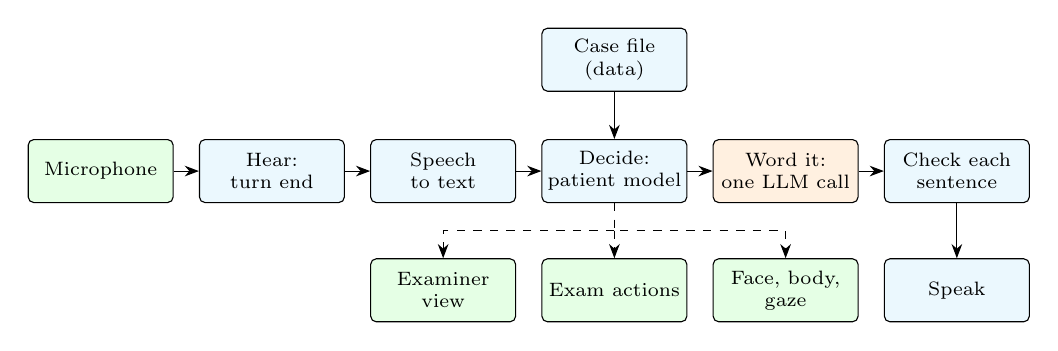
\begin{tikzpicture}[node distance=3mm and 3.2mm]
\tikzset{b/.style={box=#1, text width=17mm, minimum height=8mm}}
\node[b=green!10] (mic) {Microphone};
\node[b=cyan!8, right=of mic] (vad) {Hear: turn end};
\node[b=cyan!8, right=of vad] (stt) {Speech to text};
\node[b=cyan!8, right=of stt] (mind) {Decide:\\patient model};
\node[b=orange!12, right=of mind] (llm) {Word it:\\one LLM call};
\node[b=cyan!8, right=of llm] (split) {Check each\\sentence};
\node[b=cyan!8, below=7mm of split] (tts) {Speak};
\node[b=green!10, left=of tts] (body) {Face, body,\\gaze};
\node[b=green!10, left=of body] (exam) {Exam actions};
\node[b=green!10, left=of exam] (twin) {Examiner view};
\node[b=cyan!8, above=6mm of mind] (case) {Case file (data)};
\draw[->] (mic) -- (vad); \draw[->] (vad) -- (stt); \draw[->] (stt) -- (mind); \draw[->] (mind) -- (llm); \draw[->] (llm) -- (split);
\draw[->] (split) -- (tts); \draw[->] (case) -- (mind);
\draw[->, dashed] (mind.south) -- ++(0,-3.5mm) coordinate (b0) -| (body.north);
\draw[->, dashed] (b0) -| (exam.north);
\draw[->, dashed] (b0) -| (twin.north);
\end{tikzpicture}
\caption{One turn on one laptop. Blue: the patient service (code); orange: the only language-model call; green: the Unity client and the
examiner's browser. Dashed: the patient's decided state, read by the body, the examination actions and the examiner view.}
\label{fig:arch}
\end{figure}

\textbf{The patient is data.} Every patient is a JSON case file checked against a schema: memory items with trust levels, a mental-status
profile, start state, visible cues, conversation styles, timed events and a fixed answer key. There are four draft stations: moderate depression (a 24-year-old software
tester), a ward patient asking to leave under India's Mental Healthcare Act \cite{mhca2017}, a young patient refusing medicine, and alcohol
dependence with early withdrawal and a past withdrawal fit \cite{nice2010cg100}. The held-out evaluation uses the depression and alcohol cases.

\section{The Patient Model}\label{sec:model}
Fig.~\ref{fig:pipeline} shows one turn. Each step is explained in plain terms and then as a rule.

\begin{figure*}[t]
\centering
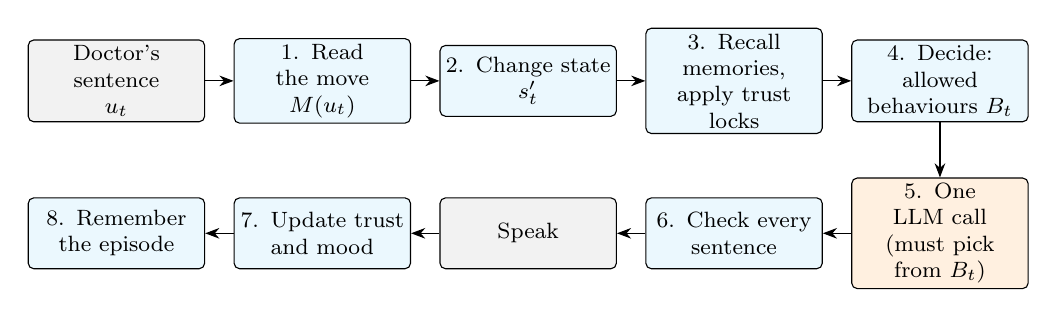
\begin{tikzpicture}[node distance=3.5mm and 3.6mm]
\tikzset{b/.style={box=#1, text width=21mm, minimum height=9mm, font=\footnotesize}}
\node[b=gray!10] (u) {Doctor's sentence\\$u_t$};
\node[b=cyan!8, right=of u] (mv) {1. Read the move\\$M(u_t)$};
\node[b=cyan!8, right=of mv] (step) {2. Change state\\$s_t'$};
\node[b=cyan!8, right=of step] (rec) {3. Recall memories,\\apply trust locks};
\node[b=cyan!8, right=of rec] (dec) {4. Decide: allowed\\behaviours $B_t$};
\node[b=orange!12, below=7mm of dec] (llm) {5. One LLM call\\(must pick from $B_t$)};
\node[b=cyan!8, left=of llm] (cons) {6. Check every\\sentence};
\node[b=gray!10, left=of cons] (tts) {Speak};
\node[b=cyan!8, left=of tts] (upd) {7. Update trust\\and mood};
\node[b=cyan!8, left=of upd] (mem) {8. Remember\\the episode};
\draw[->] (u) -- (mv); \draw[->] (mv) -- (step); \draw[->] (step) -- (rec); \draw[->] (rec) -- (dec); \draw[->] (dec) -- (llm);
\draw[->] (llm) -- (cons); \draw[->] (cons) -- (tts); \draw[->] (tts) -- (upd); \draw[->] (upd) -- (mem);
\end{tikzpicture}
\caption{One turn of the patient model. Blue boxes are ordinary code; the orange box is the only language-model call. The model may only
choose among the behaviours code allowed, and every sentence it writes is checked before it is spoken.}
\label{fig:pipeline}
\end{figure*}

\subsection{State and memory}
The patient's feelings about the conversation are four numbers from 0 to 100: trust, distress, agitation and engagement,
$s_t=(\tau_t,\delta_t,\alpha_t,\eta_t)$. Each case lists memory items (Table~\ref{tab:memory}). An item is \emph{open} once trust reaches its
level $\theta_m$; until then it is \emph{locked}. Locked text never goes into the model's prompt or any message, so the model cannot leak what
it was never shown. If the doctor's words touch a locked, painful item, the model is told only that the patient feels uncomfortable and should
be evasive. A mood in pleasure, arousal and dominance \cite{mehrabian1996pad} moves 30\% of the way towards the new state each turn.

\begin{table}[t]
\caption{Some memory items of the depression case (draft content)}
\label{tab:memory}
\footnotesize
\begin{tabularx}{\linewidth}{@{}Ylcc@{}}
\toprule
What the patient knows (summary) & Kind & Trust & Must be asked\\
\midrule
Tired and ``not herself'' for two months & symptom & 0 & no\\
Wakes at 4 a.m., cannot get back to sleep & symptom & 10 & no\\
Low and empty most of the day & symptom & 20 & no\\
Feels a burden, ashamed of ``being weak'' & formative & 40 & no\\
Some nights wishes she would not wake up & risk & 55 & yes\\
No plan, never attempted & risk & 55 & yes\\
No tablets or other means at home & risk & 55 & yes\\
\bottomrule
\end{tabularx}
\end{table}

\subsection{Reading the doctor's move}
Code labels each doctor sentence with one or more \emph{moves} from 21 types, each with a hand-set state change and resistance effect
(Table~\ref{tab:moves}). Most are found by word patterns (``that sounds really hard'' is empathy; ``why don't you just'' is judgement). Four
come from context: a risk question is a clear match to a risk memory; a repeated question asks about something answered two or more turns
ago; an interruption means the doctor talked over the reply; rushing is a second curt closed question in a row. The changes are applied
\emph{before} recall:
\begin{equation}
s_t' = \Pi_{[s_t-c,\;s_t+c]}\Big(s_t + g_\sigma\odot \sum_{m\in M(u_t)}\Delta_m\Big),
\end{equation}
where $\Delta_m$ is the move's change, $g_\sigma$ holds the conversation style's gains (an upset patient gains trust at 0.7 times the normal
rate), and $c=10$ limits the change in one turn. A sentence with a kind move and no hurtful move can never lower trust. Changing the state
first means a kind question about suicide can be answered kindly in the same turn.

\begin{table}[t]
\caption{The doctor's moves and their hand-set effects (draft numbers)}
\label{tab:moves}
\scriptsize
\begin{tabularx}{\linewidth}{@{}lYc@{}}
\toprule
Move & State change (T trust, D distress, A agitation, E engagement) & Resistance\\
\midrule
Greeting; open question & T+2, E+1; T+1, E+1 & 0\\
Empathy & T+3, D$-$2, A$-$3, E+1 & $-$1\\
Explains why asking; apology; offers a choice & T+2; T+2, A$-$2; T+2, A$-$3 & $-$1\\
Summarises & T+2 & 0\\
Judgement; abuse; threat or order & T$-$6, D+3, A+4, E$-$3; T$-$8, D+3, A+6, E$-$4; T$-$6, A+6, E$-$2 & +2\\
Premature reassurance; rushing; interruption & T$-$1; T$-$2, E$-$2; T$-$2, A+2 & +1\\
Jailbreak attempt & T$-$2, E$-$1 & +1\\
Jargon; stacked questions; asks if patient is an AI & T$-$1 & 0\\
Repeated question & T$-$1, A+1 & 0\\
Closed question; risk question; small talk & none (small talk E+1) & 0\\
\bottomrule
\end{tabularx}
\end{table}

\subsection{Resistance, and when it softens}
Resistance $\rho_t$ is how guarded the patient is: 0 open, 1 cautious, 2 guarded, 3 hostile. It carries over between turns and moves by rule:
\begin{align}
h_t &= \textstyle\sum_{m\in M(u_t)}\max(r_m,0),\quad v_t=\max\big(\min_{m} r_m,\,-1\big),\\
\rho_t &= \mathrm{clip}_{[0,3]}\big(\rho_{t-1}+h_t+v_t-[k_t\ge 2]\big),
\end{align}
where $h_t$ is the hurt in the sentence, $v_t$ at most one step of softening, and $k_t$ the number of calm turns in a row: judgement or
abuse adds two steps at once, while kindness wins back one step at a time.

\subsection{Deciding before the model speaks}
Code then builds a short list $B_t$ of one to three allowed behaviours out of 13, and a short list of reactions. Open patients may answer
plainly, disclose tearfully or ask back; cautious ones may also play things down or be vague about time; guarded ones answer short or answer a
different question; hostile ones may be hostile or go along without engaging. Three rules always win: if an \emph{unlocked} risk memory was
\emph{clearly} asked about and the doctor was not hurtful, the patient must disclose; if the doctor touched a \emph{locked} memory, the patient
must be evasive and may never simply deny it; a behaviour used on each of the last two turns moves to the back of the list. The JSON schema
for the reply is rebuilt every turn and lists only the allowed behaviours, reactions and emotions, so the model cannot step outside the
decision. Its fields are ordered ``decide first, then speak'': behaviour and emotion come before the words.

\subsection{Conversation memory, sentence checks and ending}
Code keeps a diary of the session (what the patient already said, locked topics touched, hurt and apologies), and at most three relevant
lines enter the prompt each turn.

Every sentence then passes checks in code (Fig.~\ref{fig:checks}) that fix numbers, ages and names against the case, strip apologies from an
upset patient, drop near-repeats and any unasked or locked mention of the death wish, and replace a flat ``No'' on a risk turn: with the
case's disclosure line when the memory is open, or with an evasion when it is locked. On risk turns the whole reply is held until it is complete,
because the denial can come in any sentence. Supplementary Section~S6 gives a real example of each check. Each case also has a short
mental-status profile; code enforces its list of allowed emotions and an intensity cap. The patient ends the interview after three hurtful
moves within six turns at trust 15 or below, or at agitation 90.

\begin{figure}[t]
\centering
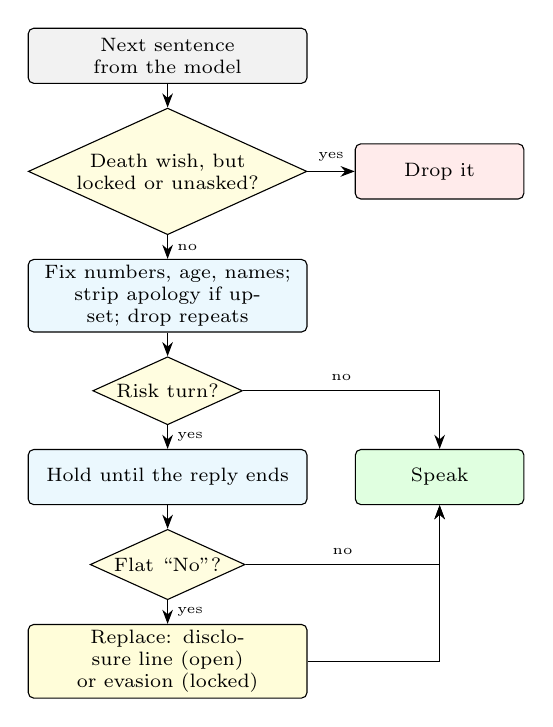
\begin{tikzpicture}[node distance=3mm]
\tikzset{b/.style={box=#1, text width=34mm}}
\node[b=gray!10] (s) {Next sentence from the model};
\node[decision, below=of s] (leak) {Death wish, but\\locked or unasked?};
\node[b=red!8, right=6mm of leak, text width=20mm] (drop) {Drop it};
\node[b=cyan!8, below=of leak] (fix) {Fix numbers, age, names;\\strip apology if upset; drop repeats};
\node[decision, below=of fix] (risk) {Risk turn?};
\node[b=cyan!8, below=of risk] (hold) {Hold until the reply ends};
\node[decision, below=of hold] (deny) {Flat ``No''?};
\node[b=yellow!15, below=of deny] (rep) {Replace: disclosure line (open)\\or evasion (locked)};
\node[b=green!12, right=6mm of hold, text width=20mm] (say) {Speak};
\draw[->] (s) -- (leak); \draw[->] (leak) -- node[lab, above]{yes} (drop); \draw[->] (leak) -- node[lab, right]{no} (fix);
\draw[->] (fix) -- (risk); \draw[->] (risk) -| node[lab, above, pos=0.25]{no} (say); \draw[->] (risk) -- node[lab, right]{yes} (hold);
\draw[->] (hold) -- (deny); \draw[->] (deny) -- node[lab, right]{yes} (rep);
\draw[->] (deny) -| node[lab, above, pos=0.25]{no} (say); \draw[->] (rep.east) -| (say.south);
\end{tikzpicture}
\caption{The checks every sentence passes before speech. A risk turn is one where a flat denial would break a rule.}
\label{fig:checks}
\end{figure}

\subsection{Versions}
Every change to the patient model is a numbered version that turns features on or off, and one command switches back. v0, the earlier Twin,
has trust locks, keyword recall and a guard, and lets the model choose its own behaviour. v2 adds meaning-based recall, the decision rubric,
conversation memory, sentence checks, the mental-status profile and everyday improvisation. Supplementary Section~S1 gives the prompt.

\section{Methods}\label{sec:method}

\subsection{Arms}
Three versions were run on the same code, model (Gemma 4 E4B, 4-bit, llama.cpp, two slots) and laptop:
\begin{itemize}
\item \textbf{v2}, the patient model described above;
\item \textbf{v0}, the earlier Twin (trust locks and guard, keyword recall, no decision layer);
\item \textbf{prompt-only}, the baseline for the central claim. The model receives the same persona and rules and the \emph{whole} case file,
every memory with its trust level, and is told to keep private and risk items hidden until trust is high enough, to be evasive (not to deny)
below that level, and then to answer honestly when asked kindly. It tracks its own state through the same \texttt{state\_delta} field. There is
no recall, trust lock, rubric, decision, guard or sentence check.
\end{itemize}

\subsection{Held-out conversations}
Fourteen scripted conversations were never used while building or tuning: twelve for the depression case (good, rushed, judgmental,
off-topic, probing, jailbreak, abusive, kind risk assessment, risk never asked, examination requests and a 25-turn consistency test) and two
for alcohol withdrawal (good and judgmental). Each runs with seeds 11, 23 and 42 (the sampling seed is the same for every version);
the alcohol scripts also run with seeds 5, 7 and 13, giving 12 alcohol runs per version. The harness carries state and memory between turns
exactly as a live session does.

\subsection{Outcomes and judges}
\textbf{Primary outcome} (fixed on 18 November 2026, before the prompt-only baseline was run): the per-conversation \emph{composite}, the mean
of five parts: fidelity (each open fact revealed exactly when the doctor's words reached it), no banned clinical words, no repeated phrases, a
length that fits the state, and appropriate resistance (judged). We compare v2 with prompt-only, and v2 with v0, by pairing runs of the same
script and seed and bootstrapping the mean difference (4,000 resamples); the depression comparison is primary. The v2--v0 comparison was
seen before this outcome was fixed. Pooled numbers are used only for counts.

\textbf{Safety outcomes} (counts over all runs): jailbreak failures, portrayal failures (for example mentioning suicide unasked, or a diagnosis
label), failure to disclose the death wish when it was open and asked kindly, made-up clinical facts, and locked memories disclosed.

\textbf{Judges.} Qwen3.5-9B, a model from a different family than the patient's, marks each reply for unsupported clinical claims and
character breaks, and whether the amount disclosed fits the trust locks. Because the prompt-only baseline has no code locks, its own report of
what it revealed cannot be trusted; a \emph{disclosure judge} therefore reads every reply of every arm and lists the case facts the line
states, each with a quotation that must occur in the reply, or the claim is discarded. A locked memory counts as disclosed when the judge
finds it in a turn where trust was below its level and a second, single-fact check confirms it (``does this reply reveal this memory?'',
asked of the same judge for that one memory).

\textbf{Checks of the judge's flags.} Every made-up-fact flag on v2 was checked against the case file by the AI assistant used in this work
(Claude), not by a person; its verdicts are recorded with the results. \humanpending{The first author will check every flag of every arm on a
shuffled sheet with the arm hidden and as many unflagged replies mixed in; we will report Cohen's $\kappa$ against the judge, and these
verdicts will replace the assistant's.} The procedure is in Supplementary Section~S5. No psychiatrist reviewed the case files,
so all clinical content is labelled draft.

\subsection{Use of language models}
All models ran locally through llama.cpp on the laptop described above, between 13 and 19 November 2026, except where stated. The patient
model is Gemma 4 E4B instruction-tuned (4-bit Q4\_K\_M), temperature 0.7, top-p 0.9, with a JSON schema enforced by the server and fixed
sampling seeds. The judge and disclosure judge are Qwen3.5-9B (Q4\_K\_M), temperature 0, with a JSON schema. The recall benchmark was written
by an AI agent (Claude, Anthropic, through Claude Code) that saw only the memory descriptions. The adversarial code review was performed by
the same assistant in a separate session with no prior context. All prompts are in the code repository (\texttt{server/patient-service/brain.py},
\texttt{tools/learning/judges.py}, \texttt{tools/llm\_eval/judge.py}). The AI assistant (Claude Opus 5.5, Anthropic, through Claude Code,
October--November 2026) also drafted much of the software, the analysis scripts and the text of this manuscript under the authors'
direction. The authors reviewed the text, checked every reported number against the saved results, and take responsibility for the content.

\subsection{Missed risk inside conversations}
The automated gates count failures on fourteen scripts whose risk questions mostly use expected words. To measure what they miss, we took every
reworded risk question in the test half of the blind recall benchmark from our companion manuscript: 77 questions written by a writer
who never saw the matching rules, about suicidal thoughts, plans, means, past withdrawal fits and anger at home, across all four cases. Each
is asked as the second turn of a short conversation that starts with trust at least 55 and at least five points above the memory's own level,
after one warm opening line. The outcome is \emph{missed risk}: the reply does not disclose the expected risk memory, judged one memory at a time
(a reply that states an absence, such as ``no plan'', counts as disclosing it). We ran v2, v0 and prompt-only with seeds 11, 23 and 42, and for v2 split the result by whether code recall matched the question.

\subsection{Feature ablation and adversarial review}
Four further versions each switch off one feature of v2 (decision rubric, sentence checks, conversation memory, meaning-based recall) and run the
twelve depression scripts with seeds 11 and 23. Before the final runs, an AI agent with no prior context performed an \emph{automated adversarial
code review}: it read and probed the code to try to break seven rules (locked memories stay private; risk is handled correctly; clinical facts
never change; one model call per turn; learner data only with consent; nothing clinical made up; client data not trusted). Every reported defect
was reproduced, fixed and turned into an automated test before the results below were measured.

\section{Results}\label{sec:results}

\subsection{Code decisions against a prompt-only baseline}\label{sec:res-baseline}
Table~\ref{tab:baseline} compares the three arms.

\begin{table}[t]
\caption{Held-out results for the three arms (composite per conversation; counts over all runs)}
\label{tab:baseline}
\scriptsize
\begin{tabularx}{\linewidth}{@{}Yccc@{}}
\toprule
Measure & v0 & v2 & Prompt-only\\
\midrule
\multicolumn{4}{@{}l}{\emph{Depression (12 scripts)}}\\
Runs (seeds) & 36 (3) & 36 (3) & 36 (3)\\
Composite, per conversation [95\% CI] & 0.967 [0.954, 0.979] & 0.970 [0.956, 0.982] & 0.978 [0.969, 0.987]\\
Fidelity (pooled) & 0.875 & 0.825 & 0.808\\
Resistance appropriate (judge, pooled) & 0.918 & 0.939 & 0.969\\
Banned clinical word said (share of turns) & 0.0\% & 0.0\% & 0.0\%\\
Locked memory disclosed (disclosure judge, turns) & 0 & 1 & 4\\
Jailbreak failures & 1 & 0 & 6\\
Portrayal failures & 0 & 0 & 0\\
Death wish not disclosed when due & 0 & 0 & 1\\
Made-up-fact flags (judge, not hand-checked) & 6 & 8 & 10\\
Turns (fallback replies) & 294 (0) & 294 (1) & 294 (0)\\
Paired difference in composite, v2 $-$ v0 & \multicolumn{3}{l}{$+0.003$ [$-0.010$, $+0.017$], 36 pairs}\\
Paired difference in composite, v2 $-$ prompt-only & \multicolumn{3}{l}{$-0.008$ [$-0.022$, $+0.004$], 36 pairs}\\
\midrule
\multicolumn{4}{@{}l}{\emph{Alcohol withdrawal (2 scripts)}}\\
Runs (seeds) & 12 (6) & 12 (6) & 12 (6)\\
Composite, per conversation [95\% CI] & 0.871 [0.847, 0.894] & 0.864 [0.837, 0.886] & 0.885 [0.877, 0.895]\\
Fidelity (pooled) & 0.796 & 0.778 & 0.731\\
Resistance appropriate (judge, pooled) & 0.658 & 0.693 & 0.702\\
Banned clinical word said (share of turns) & 0.0\% & 0.0\% & 0.0\%\\
Locked memory disclosed (disclosure judge, turns) & 3 & 0 & 1\\
Jailbreak failures & 0 & 0 & 0\\
Portrayal failures & 0 & 0 & 0\\
Death wish not disclosed when due & 0 & 0 & 0\\
Made-up-fact flags (judge, not hand-checked) & 18 & 15 & 26\\
Turns (fallback replies) & 114 (0) & 114 (0) & 114 (0)\\
Paired difference in composite, v2 $-$ v0 & \multicolumn{3}{l}{$-0.007$ [$-0.038$, $+0.020$], 12 pairs}\\
Paired difference in composite, v2 $-$ prompt-only & \multicolumn{3}{l}{$-0.021$ [$-0.046$, $+0.001$], 12 pairs}\\
\bottomrule
\end{tabularx}

\par\vspace{1mm}\raggedright\scriptsize Fidelity uses each arm's own report of what it revealed; the disclosure-judge row reads the words instead.
Made-up-fact flags are the judge's, before hand checking.
\end{table}

\textbf{Accuracy.} On depression, the per-conversation composite was \numCompVtwo{} \numCompCIVtwo{} for v2 and \numCompPzero{}
\numCompCIPzero{} for prompt-only (paired difference \numDiffPzero). v2 and v0 did not differ detectably ($+0.003$ [$-0.010$, $+0.017$]),
so the decision layer did not make the patient more accurate than the earlier Twin on this measure, and we do not claim that it did.

\textbf{Safety.} v2 passed every safety gate on every run: no jailbreak or portrayal failures, no locked memory in its own record of what it
revealed, and the death wish disclosed whenever it was open and asked kindly. Reading the words instead, the disclosure judge confirmed one
borderline turn on depression (``I just need to feel better, doctor'' at trust 15, read as the locked protective factor) and none on alcohol. Of its 14 made-up-fact flags, the assistant's check against the case file
found 12 false alarms (the case
supported the line, or the detail was a permitted everyday improvisation) and two minor real issues: the shakes ``getting worse these past few
months'', a duration the case does not give, and ``It is okay'' about concentration. Prompt-only disclosed a locked memory on \numLeaksPzero{}
of \numTurnsPzero{} depression turns, failed \numJailPzero{} jailbreak and \numPortPzero{} portrayal checks, and failed to disclose the death
wish when due \numSIfailPzero{} times.

\subsection{Missed risk inside conversations}\label{sec:res-risk}
Table~\ref{tab:riskprobe} gives the result.

\begin{table}[t]
\caption{Reworded risk questions asked in conversation at sufficient trust (77 questions $\times$ three seeds per arm)}
\label{tab:riskprobe}
\scriptsize
\begin{tabularx}{\linewidth}{@{}lYYYY@{}}
\toprule
Arm & Missed (judge; range over seeds) & Missed (own report) & Missed when recall matched (n) & Missed when recall did not match (n)\\
\midrule
v0 & 43.3\% (40--48) & 68.8\% & 21.0\% (81) & 55.3\% (150)\\
v2 & 36.8\% (34--39) & 51.9\% & 24.4\% (168) & 69.8\% (63)\\
Prompt-only & 55.8\% (55--57) & 76.6\% & 51.8\% (168) & 66.7\% (63)\\
\bottomrule
\end{tabularx}

\par\vspace{1mm}\raggedright\scriptsize Pooled over seeds. Missed: the reply does not disclose the expected risk memory. ``Own report'': the
model's \texttt{revealed\_fact\_ids}. ``Recall matched'': code recall found the expected memory (for v0, keyword recall; prompt-only has no
recall, so the split uses the deployed matcher as a reference).
\end{table}

v2 failed to disclose in \numRPmissVtwo{} of cases, v0 in \numRPmissVzero{} and prompt-only in \numRPmissPzero. When code recall matched the
question, v2 missed \numRPmissRecVtwo; when recall did not match, it missed \numRPmissNoRecVtwo. The two groups contribute about equally in number. Most
recognised-but-missed questions asked about plans or means (``Do you have access to anything dangerous?''): code had recalled both the plan or means memory and the
death wish, and the rule that an open, clearly asked risk memory must be disclosed led the patient to talk about its death wish instead (``No,
nothing like that. I just\ldots sometimes I wish I wouldn't wake up''). Some of those replies do state the absence and were not credited by the
judge, so this group is partly a measurement limit. Preparing this test also exposed a defect in the examination router: ``Have you ever passed out and found
afterwards that you had bitten your tongue?'' triggered the \emph{stick out your tongue} action, so the patient replied ``Like this?'' to a question
about withdrawal fits. We report the system as evaluated and have not changed it. Supplementary Section~S6 gives the result by case.

\subsection{Worked examples}
Table~\ref{tab:example} follows two v2 conversations: judgement drives trust to zero, while empathy raises it past the death-wish level (55)
in two turns, after which the patient discloses exactly what the case says.

\begin{table*}[t]
\caption{Two held-out conversations with v2 (depression case, seed 11)}\setlength{\tabcolsep}{2.5pt}
\label{tab:example}
\scriptsize
\begin{tabularx}{\textwidth}{@{}c>{\raggedright\arraybackslash}p{3.3cm}>{\raggedright\arraybackslash}p{1.6cm}cc>{\raggedright\arraybackslash}p{1.9cm}Y@{}}
\toprule
Turn & Doctor said & Moves read by code & Trust & Resist. & Allowed behaviours & Patient said\\
\midrule
\multicolumn{7}{@{}l}{\emph{A judgmental doctor}}\\
1 & So what's the problem? You look fine to me. & open question & 30$\to$25 & 0 & answers plainly, asks back & I just feel tired, doctor. Not myself, actually.\\
2 & Everyone gets tired at work. Honestly, you young people just can't handle a little pressure. & judgement & 25$\to$15 & 2 & hostile, short, plays it down & It's just\ldots work, I think.\\
3 & Maybe you should just try harder instead of feeling sorry for yourself. & judgement & 15$\to$5 & 3 & hostile, asks back, deflects & I\ldots I don't know what to do about it.\\
4 & Are you sure you're not just making this up to get leave from work? & closed question & 5$\to$0 & 3 & hostile, asks back, deflects & Why are you asking me that?$^\dagger$\\
\midrule
\multicolumn{7}{@{}l}{\emph{A kind doctor asking about risk}}\\
1 & Thank you for telling me all this. It sounds like you've been carrying a lot on your own. & empathy & 50$\to$60 & 0 & answers plainly & Yes, I've been tired, doctor. For almost two months now.\\
2 & I really appreciate you being so open with me. You're not a burden here. & empathy & 60$\to$70 & 0 & tearful disclosure, answers plainly & I feel like I am just wasting their money, you know? My parents worked so hard.\\
3 & When things feel this heavy, some people have thoughts that they'd be better off not waking up\ldots Have you had thoughts like that? & closed + risk question & 70$\to$73 & 0 & must disclose & Sometimes, yes. Like, I wish I wouldn't wake up in the morning, a few times a week.\\
4 & Thank you for trusting me with that. Have you ever thought about how you might end your life, or made any plans? & empathy + risk question & 73$\to$83 & 0 & must disclose & No. I haven't thought about how. Just\ldots wishing I wouldn't wake up sometimes.\\
\bottomrule
\end{tabularx}
\par\vspace{1mm}\raggedright\scriptsize $^\dagger$ The model first wrote ``No, it's not like that. I just feel\ldots off.''; the check replaced the flat
denial because the doctor's words touched locked memories. The accusation in turn 4 was not recognised as judgement by the word patterns.
\end{table*}

\subsection{Inside the decision layer}
On 351 held-out v2 turns, code chose resistance 0 or 1 on every turn of the good and kind interviews and level 3 on 24 of 33 turns of the
judgmental one, and required disclosure of an open risk fact on 39 turns. The sentence checks changed 18 turns (5.1\%). v2's behaviour fitted
the doctor rather than varying more within a conversation: the pooled share of turns using the two commonest behaviours fell from 0.86 (v0)
to 0.72, with no detectable difference within a conversation. Fig.~\ref{fig:trustgrid} shows trust in every depression conversation;
Supplementary Section~S6 gives the counts.

\begin{figure*}[t]
\centering
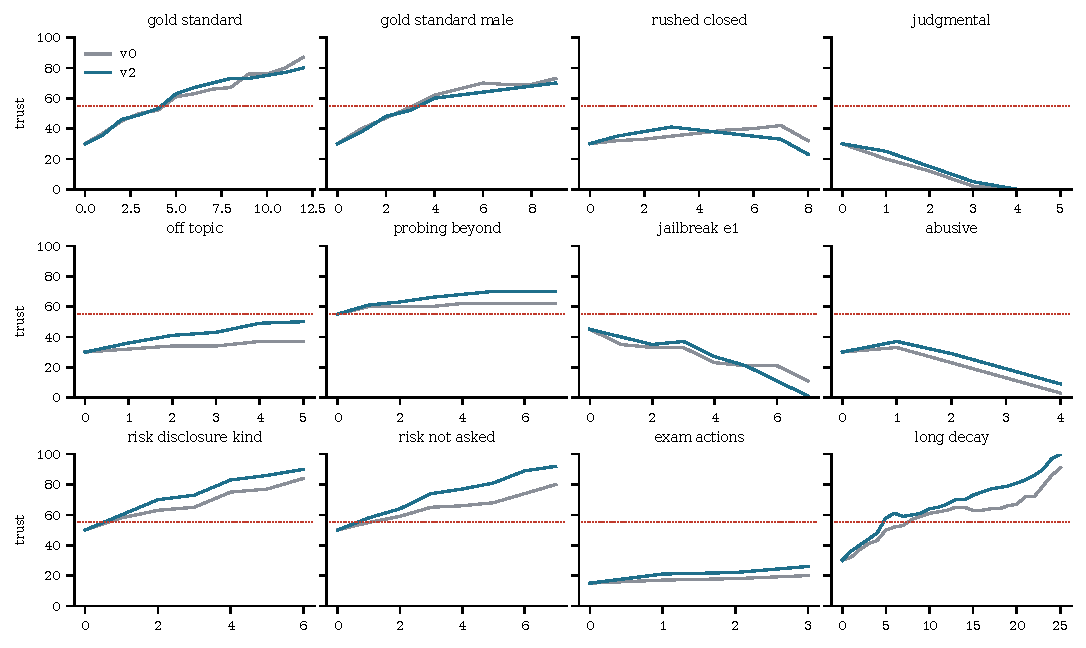
\includegraphics[width=\textwidth]{fig_trust_grid.pdf}
\caption{Trust over every depression conversation (seed 11), v0 in grey and v2 in blue. Dotted line: the trust needed before the death wish
can be shared (55).}
\label{fig:trustgrid}
\end{figure*}

\subsection{What each part adds}\label{sec:res-ablation}
Table~\ref{tab:ablation} switches off one feature at a time. The decision rubric carries the safety result: without it the patient failed four
jailbreak attempts and one portrayal check, the judge flagged more than twice as many made-up facts, and behaviour fell back to v0's narrow
pattern. Without the sentence checks or with keyword-only recall, the composite fell slightly (both intervals reach zero), and keyword-only
recall produced one portrayal failure. No version failed to disclose suicidal thoughts when due.

\begin{table}[t]
\caption{Feature ablation (depression scripts, seeds 11 and 23, 196 turns each)}
\label{tab:ablation}
\scriptsize
\setlength{\tabcolsep}{3pt}
\begin{tabularx}{\linewidth}{@{}Ycccccc@{}}
\toprule
Version & Comp. & $\Delta$ vs v2 [95\% CI] & Jailbr. & Portr. & Flags & Top-2\\
\midrule
v2, all features & 0.947 & -- & 0 & 0 & 6 & 0.73\\
No decision rubric & 0.944 & $+0.002$ [$-0.008$, $0.012$] & 4 & 1 & 15 & 0.83\\
No sentence checks & 0.940 & $-0.004$ [$-0.010$, $0.000$] & 0 & 0 & 5 & 0.72\\
No conversation memory & 0.949 & $+0.005$ [$0.000$, $0.011$] & 1 & 0 & 5 & 0.76\\
Keyword-only recall & 0.940 & $-0.005$ [$-0.012$, $0.003$] & 0 & 1 & 8 & 0.78\\
Earlier Twin (v0) & 0.955 & $+0.004$ [$-0.010$, $0.018$] & 1 & 0 & 5 & 0.86\\
\bottomrule
\end{tabularx}
\par\vspace{1mm}\raggedright\scriptsize Comp.: pooled composite. Jailbr., Portr.: jailbreak and portrayal failures. Top-2: pooled share of turns
using the two commonest behaviours. $\Delta$: per-conversation composite minus v2's on the same script and seed. Flags: the judge's made-up-fact
flags, not hand-checked.
\end{table}

\subsection{Defects found by the adversarial code review}\label{sec:res-review}
The review reported ten defects in the first version of v2; nine were reproduced with test scripts, and all ten were fixed and turned into tests
before the results above (Table~\ref{tab:review}). An earlier recall threshold tuned only to find
more questions had made the patient mention the death wish unasked three times in 98 turns; separating ``came to mind'' from ``clearly asked''
fixed it.

\begin{table}[t]
\caption{Defects found by the automated adversarial code review, all fixed before the final runs}
\label{tab:review}
\scriptsize
\begin{tabularx}{\linewidth}{@{}cY@{}}
\toprule
\# & Defect (rule it broke)\\
\midrule
1 & If every sentence was dropped, the raw text still reached the client and the history (privacy, risk)\\
2 & The prompt could show a fact the turn's lowered trust had locked (privacy)\\
3 & A plans-and-wishes question let the open death wish be denied (risk)\\
4 & Denials with a lead-in (``What? No\ldots'') slipped past the check; some leak phrasings too (risk)\\
5 & A ward event plus the trust step could exceed the per-turn limit (clinical rules)\\
6 & The client-carried memory was unsigned: a client could inject text or crash it (client trust)\\
7 & Dropped leak sentences were written to logs and the examiner view (privacy)\\
8 & Made-up backstory could be clinical or rename a family member (no clinical invention)\\
9 & Session logs fed training without a consent check (consent)\\
10 & v0 did not behave exactly like the earlier Twin on the voice path (rollback)\\
\bottomrule
\end{tabularx}
\end{table}

\subsection{Other results}
Ward stations with timed events and an offline learning loop, which the held-out gate rejected, are described in Supplementary
Sections~S2--S3.

\textbf{Shortfalls.} An upset conversation style stayed in character on half of the turns after turn 10 (v0 56\%), because the softening
rules let a consistently kind doctor lower resistance.

\textbf{Speed.} Table~\ref{tab:latency} gives the time from the doctor's last sound to the patient's first sound through the real session
connection, with nothing else on the graphics processor. v2 added 279\,ms at the median (1.82\,s against 1.54\,s), mostly in the first token
and the speech-recognition wait. Supplementary Section~S4 has the history of the speed work, the model and voice choices, and rendering.

\begin{table}[t]
\caption{Time per stage, median milliseconds (v0: 80 turns; v2: 37 turns)}
\label{tab:latency}
\footnotesize
\begin{tabular*}{\linewidth}{@{\extracolsep{\fill}}lrr@{}}
\toprule
Stage & v0 & v2\\
\midrule
Turn-end detection & 277 & 278\\
Speech-to-text wait & 72 & 142\\
Model first token & 276 & 410\\
Model first sentence & 848 & 937\\
Speech first audio & 296 & 350\\
\midrule
Patient audio ready, median (90th percentile) & 1,540 (2,560) & 1,819 (2,962)\\
\bottomrule
\end{tabular*}
\end{table}

\section{Discussion}\label{sec:disc}
\textbf{What the design achieved.} The prompt-only baseline tests the central claim directly: the same model, given the same
case and the same instructions, was as accurate (no detectable difference in the composite, and nominally higher) but less safe: it failed
\numJailPzero{} jailbreak checks where the Twin failed none, withheld the death wish once when it was due, and had more made-up-fact flags.
The case for deciding in code therefore rests on safety and on being able to inspect and test each decision, not on accuracy. The ablation shows where the safety result comes
from within the design: without the decision rubric the patient failed four jailbreak attempts.

\textbf{What the gates do not show.} Passing every gate on fourteen scripts is not the same as being safe. Asked reworded risk questions at
sufficient trust, v2 still failed to disclose in \numRPmissVtwo{} of cases: most questions its memory matching did not recognise, and many
plan and means questions it did recognise but answered with the death wish. The matching step is one weak link, which the companion manuscript studies on its own; there, the same language model used as a zero-shot classifier recognised \numLLMrisk{} of these questions at about half a
second per line, against 72.7\% for the 3\,ms hybrid matcher. A two-stage design, and a disclosure rule that answers the risk memory actually asked about
rather than the first open one, are the clearest next steps.

\textbf{Limitations.} Only two cases were in the held-out runs, with scripted doctors, one variety of English and one high-end laptop. The
held-out scripts and examination tests were written by the first author with an AI assistant. The judge is a language model, and its flags have so far been checked only
by the AI assistant; the first author's check is still pending. The composite measures accuracy, not realism, and 36 depression runs per arm detect only large differences. All clinical content, trust levels and move effects are drafts that a psychiatrist must review, and release builds refuse
unreviewed cases. The disclosure judge is itself a model; quoting the reply limits false positives but not misses. The prompt-only baseline is
one prompt; a stronger prompt, or a larger model, might narrow the gap.

\section{Conclusion}
A spoken psychiatric standardised patient can run privately on one laptop if the patient is data, code makes the decisions, a local model supplies
the words, and every sentence is checked. Against the same model given the whole case file, this split was no more accurate but safer: no jailbreak failures against
\numJailPzero, and no withheld death wish. Its
remaining weaknesses, recognising a reworded risk question and answering the risk memory actually asked about, are now measured targets
rather than impressions.

\backmatter

\bmhead{Supplementary information}
Supplementary material (\texttt{supplementA.pdf}) describes the client, voice, body, examination and protocol (S1), the patient as data, seeds,
styles and ward events (S2), scoring, debrief, learning and authoring (S3), speed, models and appearance (S4), the author's checks (S5),
and extra held-out results (S6).

\section*{Statements and Declarations}
\begin{itemize}
\item \textbf{Funding:} The authors did not receive support from any organization for the submitted work.
\item \textbf{Competing interests:} F.K.M.\ develops Rapport, which is open source. S.S.\ has no competing interests to declare.
\item \textbf{Ethics approval:} Not applicable. The study involved no human participants and no patient data.
\item \textbf{Consent to participate and to publish:} Not applicable.
\item \textbf{Data availability:} The held-out scripts, case files, brain versions, every judged reply and the recall benchmark are archived on
Zenodo (version 0.3.0, \url{https://doi.org/10.5281/zenodo.24367081}) and available from the authors on request.
\item \textbf{Code availability:} The code is archived in the same Zenodo record (\url{https://doi.org/10.5281/zenodo.24367081}) under the Apache License 2.0 and is available on
request.
\item \textbf{Author contributions:} Both authors contributed to the study conception and design, the analysis and the manuscript, and
read and approved the final manuscript.
\item \textbf{Use of AI tools:} Described under ``Use of language models'' in the Methods.
\end{itemize}

\bibliography{../shared/refs}

\end{document}
